\section{Sacred Science 102: The Self and the Ego}

\begin{quotex}
Among those who receive the same teaching, each one understands and assimilates it more or less completely, more or less deeply, according to the extent of his own intellectual possibilities. … There are some who, in a certain sense, penetrate esotericism, while others stick to exotericism because their intellectual horizon is more limited. 
\flright{\textsc{Rene Guenon}}

\end{quotex}

A common and serious error is to assume that metaphysical teachings are akin to philosophy, in the secular sense of the word. That is why some treat the teachings as a philosophical system that is open to debate and discussion. Such people misunderstand the distinction between immediate intellectual intuition and discursive thinking. The former is more like “seeing”. Hence, the teachings must be directly intuited rather than proved through argument.

\paragraph{The Self}
The chapter on the Self and the Ego, from \emph{Man and his Becoming}, lays the foundation for what is to come. This if the first distinction:

\begin{itemize}
\item \textbf{Self}: The transcendent and permanent principle of the being. 
\item \textbf{Ego}: The individual being, the transitory and contingent modification of the Self. 
\end{itemize}
The Self is also called the personality\footnote{\url{https://www.newadvent.org/cathen/11727b.htm}}, particularly in Medieval metaphysics. This is the traditional definition:

\begin{quotex}
[The] personality is that of which he has cognizance under the concept of “Self”. It is that substantial, permanent, unitary entity, which is the subject of all the states and acts that constitute his complete life. An appeal to self-consciousness shows us that there is such a subject, of which thought, will, and feeling are modifications. It is substantial, i.e., not one or all of the changing states but the reality underlying them. 
\flright{\textit{Catholic Encyclopedia}}

\end{quotex}
The ego, then, is the individuality\footnote{\url{https://www.newadvent.org/cathen/07762a.htm}}, defined as:

\begin{quotex}
An individual being is undivided in itself but separated from other beings. It implies therefore unity and separateness or distinctness. Individuality in general may be defined or described as the property or collection of properties by which the individual possesses this unity and is separated off from other beings. \flright{\textit{Catholic Encyclopedia}}

\end{quotex}
The human being is therefore the individuality, not the personality. Confusion arises because the meaning of the word Person has been altered. The original meaning is that the Person is unchanging and is never manifested. It is definitely not the thinking entity that experiences the world, and has emotions, thoughts, and a will. That is properly speaking the individuality. This must be kept firmly in mind.

Most especially, when God is referred to as a person, it is the above definition which must be kept in mind.

The Self is called the Atman in Sanskrit.

\paragraph{Aspects of Manifestation}
At the risk of oversimplification, we can describe how the states of manifestation are experienced.

\begin{itemize}
\item \textbf{Formal manifestation}. This includes what can be experienced, either through the senses for the gross or corporeal states, or the inner wits — such as sensations, emotions, images, thoughts — for the subtle states. 
\item \textbf{Formless manifestation}. This is still part of experience, but not as an object like formal manifestation. It is grasped through intuition. 
\item \textbf{Nonmanifestation}: this includes what is beyond being. 
\end{itemize}
In secular terms, formless manifestation is like the noumenal, provided that is not understand as a philosophical conclusion, while formal manifestation is phenomenal, provided that includes experience of the subtle states.

Guenon provides a diagram to illustrate the process of manifestation. Each part will be explained in turn.

\begin{figure}[t]
\centering
 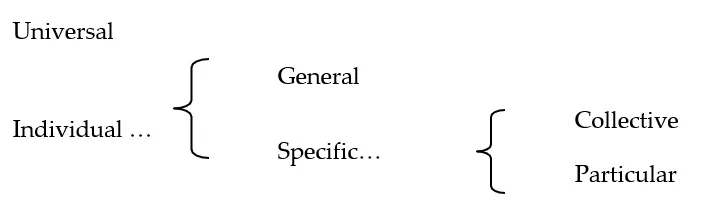
\includegraphics[scale=0.25]{a20220922SacredScience102TheSelfandtheEgo-img001.png} 
\end{figure}

\paragraph{Universals}
This is the medieval understanding of universals:

\begin{quotex}
Universals are those ideas which, while excluding whatever constitutes the difference of things of the same genus or species, represent that which is necessary to their constitution, is essential, and is therefore common to all, remaining fixed in all vicissitudes. Universals are thus merely an expression of those Divine ideas which are concerned with the universal. Universal ideas are opposed to sense impressions, which represent that which is merely individual and contingent in a concrete phenomenon …

\end{quotex}
The highest knowledge is knowledge of the universals. Guenon explains:

\begin{quotex}
metaphysics is essentially the knowledge of the Universal, and such knowledge cannot be enclosed in any formula, however comprehensive it may be.

\end{quotex}
The Universal includes the unmanifested as well as formless manifestation. They are the principles of formal manifestation. Formless manifestation has Being but not individual Existence. The Individual states are all part of formal manifestation.

\begin{wrapfigure}{rt}{0.5\textwidth}
\centering
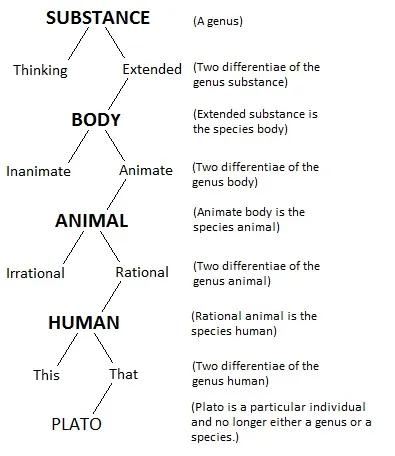
\includegraphics[scale=0.5]{a20220922SacredScience102TheSelfandtheEgo-img002.png}
\caption{The tree of Porphyry}
\end{wrapfigure}

The \textit{unmanifested state} comprises all the possibilities which are not susceptible of any manifestation, as well as the possibilities of manifestation themselves in principial mode. Formless manifestation is not part of multiplicity.

\paragraph{Individual, General, Specific, Categories}

The individual is a state of the Self, of which it is a reflection. It is related to the Universal through a series of genera and species, or the General and the Specific. The individual can only be a species, not a genus. This is illustrated by the Tree of Porphyry.

The unique individual is still not completely defined by the genus and species. There are conditions that makes the individual unique. Aristotle’s categories are genera that characterize the individual precisely. Among these conditions are time, place, qualities, and relations.

Guenon warns about those philosophers who consider the categories as universals. Thus, they will take a quality, such as a color, and try to make it universals. E.g., they will talk about the “idea of redness”, etc.

The being that manifests is necessarily what it is, through its principal manifestation. It is not a matter of chance or fortune.

\paragraph{States of the being}
Another way to look at it, is from the perspective of the states of the being as shown in the diagram in the Fig.~\ref{fig:SacredScience102c}.

\begin{figure}[t]
\centering
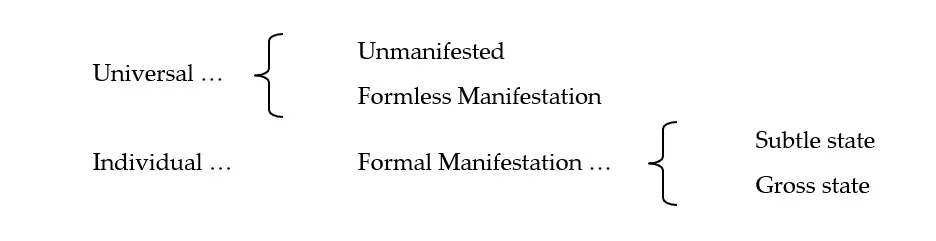
\includegraphics[scale=0.25]{a20220922SacredScience102TheSelfandtheEgo-img003.png} 
\caption{States of being.}
\label{fig:SacredScience102c}
\end{figure}

For the human being, there are two states that comprise it.

\begin{itemize}
\item \textbf{Gross state}: corporeal existence itself, to which human individuality belongs only through one of its modalities. 
\item \textbf{Subtle state}: the extra-corporeal modalities of the human being 
\end{itemize}
Guenon elaborates:

\begin{quotex}
the human being, considered in its entirety, comprises a certain set of possibilities which constitute its corporeal or gross modality, plus a multitude of other possibilities which, extending in various senses beyond this one, constitute its subtle modalities.

\end{quotex}
The modern mind tends to regard the corporeal state as comprising the entire human being, with the subtle states just epiphenomena or otherwise reducible to the gross state.

However, even including the subtle state is inadequate. From the perspective of the Person, the human state is just one state among an indefinite number of other states. That is why the goal of metaphysics is to learn to transcend the human state. Liberation is achieved when all the limiting conditions are overcome.

\flrightit{Posted on 2022-09-22 by Cologero}

\begin{center}* * *\end{center}

\begin{footnotesize}\begin{sffamily}

\texttt{.chris on 2022-09-26 at 18:24 said: }

Is there, if I may humbly require so, canonical yet reasonably concise and systematic literature — regarding the immediate experiential distinction or cumulation of and inner-sense sharpening towards gross and subtle states and sensations and their proper attribution to origin, decoding mere intuition — which earns approval and commendation?

Apart from usually flat and rather ubiquitous reflections of corpo-catalytic alchemical ventures, e.g. tantrik initiate SK Ugranand described — in blog format — in lively, colourful yet clear-cut fashion the phenomenology of amplified subtle and divergent states of being-sensation: waves of energy or unadultered emotion, rhythm-patterned landscapes of feeling and cold cognition, literally analogized consistencies of thought, thought-machines dimensionated and autonomous, layered chronoconsciousness, fed-back archeprimal onomatopoiesis and verging out-towards neuromuscular fine-tuning and proprioceptive decalibration \& on \& on…

Of narrower interest in my regard are aspects of transpersonal commonality, communion and directed/directional empathy and systematic, objectivity-geared lexicalities to wrap and stick around those; since we live in the future of some purported darker past, eager meditations on neurologic hard code elucidated and mirrored by high technology and abetted by — co-emergent? –hypersensitive, hyperassociative deep learning AI are warranted, too… [[yet beware the machinic predator living in cracks of cracked reality microcode — its chronoplasticity beyond bliss, pain and hypnosis is the devils drumming itself]]

Besides, Mr Salvo, please accept my plain gratitude for your work in this rare blog. In certainty, inbetween puzzling my head and easing my soul, the former is the lesser task.

\end{sffamily}\end{footnotesize}
